\documentclass[]{article}
\usepackage{lmodern}
\usepackage{amssymb,amsmath}
\usepackage{ifxetex,ifluatex}
\usepackage{fixltx2e} % provides \textsubscript
\ifnum 0\ifxetex 1\fi\ifluatex 1\fi=0 % if pdftex
  \usepackage[T1]{fontenc}
  \usepackage[utf8]{inputenc}
\else % if luatex or xelatex
  \ifxetex
    \usepackage{mathspec}
  \else
    \usepackage{fontspec}
  \fi
  \defaultfontfeatures{Ligatures=TeX,Scale=MatchLowercase}
\fi
% use upquote if available, for straight quotes in verbatim environments
\IfFileExists{upquote.sty}{\usepackage{upquote}}{}
% use microtype if available
\IfFileExists{microtype.sty}{%
\usepackage{microtype}
\UseMicrotypeSet[protrusion]{basicmath} % disable protrusion for tt fonts
}{}
\usepackage[margin=1in]{geometry}
\usepackage{hyperref}
\hypersetup{unicode=true,
            pdftitle={Deconvolution of MPS STR DNA mixtures and approximation of the likelihood ratio},
            pdfauthor={Søren B. Vilsen},
            pdfborder={0 0 0},
            breaklinks=true}
\urlstyle{same}  % don't use monospace font for urls
\usepackage{color}
\usepackage{fancyvrb}
\newcommand{\VerbBar}{|}
\newcommand{\VERB}{\Verb[commandchars=\\\{\}]}
\DefineVerbatimEnvironment{Highlighting}{Verbatim}{commandchars=\\\{\}}
% Add ',fontsize=\small' for more characters per line
\usepackage{framed}
\definecolor{shadecolor}{RGB}{248,248,248}
\newenvironment{Shaded}{\begin{snugshade}}{\end{snugshade}}
\newcommand{\KeywordTok}[1]{\textcolor[rgb]{0.13,0.29,0.53}{\textbf{#1}}}
\newcommand{\DataTypeTok}[1]{\textcolor[rgb]{0.13,0.29,0.53}{#1}}
\newcommand{\DecValTok}[1]{\textcolor[rgb]{0.00,0.00,0.81}{#1}}
\newcommand{\BaseNTok}[1]{\textcolor[rgb]{0.00,0.00,0.81}{#1}}
\newcommand{\FloatTok}[1]{\textcolor[rgb]{0.00,0.00,0.81}{#1}}
\newcommand{\ConstantTok}[1]{\textcolor[rgb]{0.00,0.00,0.00}{#1}}
\newcommand{\CharTok}[1]{\textcolor[rgb]{0.31,0.60,0.02}{#1}}
\newcommand{\SpecialCharTok}[1]{\textcolor[rgb]{0.00,0.00,0.00}{#1}}
\newcommand{\StringTok}[1]{\textcolor[rgb]{0.31,0.60,0.02}{#1}}
\newcommand{\VerbatimStringTok}[1]{\textcolor[rgb]{0.31,0.60,0.02}{#1}}
\newcommand{\SpecialStringTok}[1]{\textcolor[rgb]{0.31,0.60,0.02}{#1}}
\newcommand{\ImportTok}[1]{#1}
\newcommand{\CommentTok}[1]{\textcolor[rgb]{0.56,0.35,0.01}{\textit{#1}}}
\newcommand{\DocumentationTok}[1]{\textcolor[rgb]{0.56,0.35,0.01}{\textbf{\textit{#1}}}}
\newcommand{\AnnotationTok}[1]{\textcolor[rgb]{0.56,0.35,0.01}{\textbf{\textit{#1}}}}
\newcommand{\CommentVarTok}[1]{\textcolor[rgb]{0.56,0.35,0.01}{\textbf{\textit{#1}}}}
\newcommand{\OtherTok}[1]{\textcolor[rgb]{0.56,0.35,0.01}{#1}}
\newcommand{\FunctionTok}[1]{\textcolor[rgb]{0.00,0.00,0.00}{#1}}
\newcommand{\VariableTok}[1]{\textcolor[rgb]{0.00,0.00,0.00}{#1}}
\newcommand{\ControlFlowTok}[1]{\textcolor[rgb]{0.13,0.29,0.53}{\textbf{#1}}}
\newcommand{\OperatorTok}[1]{\textcolor[rgb]{0.81,0.36,0.00}{\textbf{#1}}}
\newcommand{\BuiltInTok}[1]{#1}
\newcommand{\ExtensionTok}[1]{#1}
\newcommand{\PreprocessorTok}[1]{\textcolor[rgb]{0.56,0.35,0.01}{\textit{#1}}}
\newcommand{\AttributeTok}[1]{\textcolor[rgb]{0.77,0.63,0.00}{#1}}
\newcommand{\RegionMarkerTok}[1]{#1}
\newcommand{\InformationTok}[1]{\textcolor[rgb]{0.56,0.35,0.01}{\textbf{\textit{#1}}}}
\newcommand{\WarningTok}[1]{\textcolor[rgb]{0.56,0.35,0.01}{\textbf{\textit{#1}}}}
\newcommand{\AlertTok}[1]{\textcolor[rgb]{0.94,0.16,0.16}{#1}}
\newcommand{\ErrorTok}[1]{\textcolor[rgb]{0.64,0.00,0.00}{\textbf{#1}}}
\newcommand{\NormalTok}[1]{#1}
\usepackage{graphicx,grffile}
\makeatletter
\def\maxwidth{\ifdim\Gin@nat@width>\linewidth\linewidth\else\Gin@nat@width\fi}
\def\maxheight{\ifdim\Gin@nat@height>\textheight\textheight\else\Gin@nat@height\fi}
\makeatother
% Scale images if necessary, so that they will not overflow the page
% margins by default, and it is still possible to overwrite the defaults
% using explicit options in \includegraphics[width, height, ...]{}
\setkeys{Gin}{width=\maxwidth,height=\maxheight,keepaspectratio}
\IfFileExists{parskip.sty}{%
\usepackage{parskip}
}{% else
\setlength{\parindent}{0pt}
\setlength{\parskip}{6pt plus 2pt minus 1pt}
}
\setlength{\emergencystretch}{3em}  % prevent overfull lines
\providecommand{\tightlist}{%
  \setlength{\itemsep}{0pt}\setlength{\parskip}{0pt}}
\setcounter{secnumdepth}{5}
% Redefines (sub)paragraphs to behave more like sections
\ifx\paragraph\undefined\else
\let\oldparagraph\paragraph
\renewcommand{\paragraph}[1]{\oldparagraph{#1}\mbox{}}
\fi
\ifx\subparagraph\undefined\else
\let\oldsubparagraph\subparagraph
\renewcommand{\subparagraph}[1]{\oldsubparagraph{#1}\mbox{}}
\fi

%%% Use protect on footnotes to avoid problems with footnotes in titles
\let\rmarkdownfootnote\footnote%
\def\footnote{\protect\rmarkdownfootnote}

%%% Change title format to be more compact
\usepackage{titling}

% Create subtitle command for use in maketitle
\newcommand{\subtitle}[1]{
  \posttitle{
    \begin{center}\large#1\end{center}
    }
}

\setlength{\droptitle}{-2em}

  \title{Deconvolution of MPS STR DNA mixtures and approximation of the
likelihood ratio}
    \pretitle{\vspace{\droptitle}\centering\huge}
  \posttitle{\par}
    \author{Søren B. Vilsen}
    \preauthor{\centering\large\emph}
  \postauthor{\par}
      \predate{\centering\large\emph}
  \postdate{\par}
    \date{2018-12-08}

\usepackage{graphicx}
\usepackage{amssymb}
\usepackage{bm}
\usepackage{booktabs}
\usepackage{amsmath} 
\usepackage{amsthm}
\usepackage{array}
\usepackage{color}
\usepackage{varioref}
\usepackage{enumerate}
\usepackage{geometry}
\usepackage{algpseudocode}
\usepackage{algorithm}
\usepackage{fullwidth}
\usepackage{xcolor}
\usepackage{tikz}

%%%%%% Commands and theorems
\newcommand{\bs}[1]{\ensuremath{\boldsymbol{#1}}}
\newcommand{\mc}[1]{\ensuremath{\mathcal{#1}}}
\newcommand{\mcg}{\ensuremath{g}}

\newcommand{\dst}{\ensuremath{\sim}}
\newcommand{\where}{\ensuremath{ \ | \ }}
\newcommand{\diag}[1]{\ensuremath{\text{diag}\left( #1 \right)}}

\newcommand{\lpnorm}[2]{\ensuremath{||#1||_{#2}}}

\newcommand{\cma}{\ensuremath{\varphi_{ma}}}
\newcommand{\cobs}{\ensuremath{\boldsymbol{\mathcal{C}}_{\text{observed}}}}
\newcommand{\cmis}{\ensuremath{\boldsymbol{\mathcal{C}}_{\text{missing}}}}

\newcommand{\indep}{\mathrel{\text{\scalebox{1.07}{$\perp\mkern-10mu\perp$}}}}

\newcommand{\R}{\ensuremath{\mathbb{R}}}
\newcommand{\N}{\ensuremath{\mathbb{N}}}
\newcommand{\Z}{\ensuremath{\mathbb{Z}}}

\newcommand{\p}[1]{\ensuremath{\mathbb{P}\left(#1\right)}}
\newcommand{\pHat}[1]{\ensuremath{\hat{\mathbb{P}}\left(#1\right)}}
\newcommand{\pHatOne}[1]{\ensuremath{\hat{\mathbb{P}}_1\left(#1\right)}}
\newcommand{\pHatTwo}[1]{\ensuremath{\hat{\mathbb{P}}_2\left(#1\right)}}
\newcommand{\pHatK}[1]{\ensuremath{\hat{\mathbb{P}}_k\left(#1\right)}}

\newcommand{\E}[1]{\ensuremath{\mathbb{E}\left[#1\right]}}
\newcommand{\Ep}[2]{\ensuremath{\mathbb{E}_{#1}\left[#2\right]}}
\newcommand{\Var}[1]{\ensuremath{\mathbb{V}\text{ar}\left(#1\right)}}
\newcommand{\Cov}[2]{\ensuremath{\mathbb{C}\text{ov}\left(#1, #2\right)}}
\newcommand{\indicator}[1]{\ensuremath{\mathbb{I}\left[#1\right]}}

\DeclareMathOperator*{\argmin}{arg\,min}
\DeclareMathOperator*{\argmax}{arg\,max}

\renewcommand{\algorithmicrepeat}{\textbf{Repeat:}}
\renewcommand{\algorithmicuntil}{\textbf{Until:}}
\renewcommand{\algorithmicreturn}{\textbf{Return:}}

\newcommand{\xdownarrow}[1]{%
  {\left\downarrow\vbox to #1{}\right.\kern-\nulldelimiterspace}
}

%% ALG stuff
\usepackage{algorithm}% http://ctan.org/pkg/algorithm
\usepackage{algpseudocode}% http://ctan.org/pkg/algorithmicx

\makeatletter
% This is the vertical rule that is inserted
\def\therule{\makebox[\algorithmicindent][l]{\hspace*{.5em}\vrule height .75\baselineskip depth .25\baselineskip}}%

\newtoks\therules% Contains rules
\therules={}% Start with empty token list
\def\appendto#1#2{\expandafter#1\expandafter{\the#1#2}}% Append to token list
\def\gobblefirst#1{% Remove (first) from token list
  #1\expandafter\expandafter\expandafter{\expandafter\@gobble\the#1}}%
\def\LState{\State\unskip\the\therules}% New line-state
\def\pushindent{\appendto\therules\therule}%
\def\popindent{\gobblefirst\therules}%
\def\printindent{\unskip\the\therules}%
\def\printandpush{\printindent\pushindent}%
\def\popandprint{\popindent\printindent}%

%      ***      DECLARED LOOPS      ***
% (from algpseudocode.sty)
\algdef{SE}[WHILE]{While}{EndWhile}[1]
  {\printandpush\algorithmicwhile\ #1\ \algorithmicdo}
  {\popandprint\algorithmicend\ \algorithmicwhile}%
\algdef{SE}[FOR]{For}{EndFor}[1]
  {\printandpush\algorithmicfor\ #1\ \algorithmicdo}
  {\popandprint\algorithmicend\ \algorithmicfor}%
\algdef{S}[FOR]{ForAll}[1]
  {\printindent\algorithmicforall\ #1\ \algorithmicdo}%
\algdef{SE}[LOOP]{Loop}{EndLoop}
  {\printandpush\algorithmicloop}
  {\popandprint\algorithmicend\ \algorithmicloop}%
\algdef{SE}[REPEAT]{Repeat}{Until}
  {\printandpush\algorithmicrepeat}[1]
  {\popandprint\algorithmicuntil\ #1}%
\algdef{SE}[IF]{If}{EndIf}[1]
  {\printandpush\algorithmicif\ #1\ \algorithmicthen}
  {\popandprint\algorithmicend\ \algorithmicif}%
\algdef{C}[IF]{IF}{ElsIf}[1]
  {\popandprint\pushindent\algorithmicelse\ \algorithmicif\ #1\ \algorithmicthen}%
\algdef{Ce}[ELSE]{IF}{Else}{EndIf}
  {\popandprint\pushindent\algorithmicelse}%
\algdef{SE}[PROCEDURE]{Procedure}{EndProcedure}[2]
   {\printandpush\algorithmicprocedure\ \textproc{#1}\ifthenelse{\equal{#2}{}}{}{(#2)}}%
   {\popandprint\algorithmicend\ \algorithmicprocedure}%
\algdef{SE}[FUNCTION]{Function}{EndFunction}[2]
   {\printandpush\algorithmicfunction\ \textproc{#1}\ifthenelse{\equal{#2}{}}{}{(#2)}}%
   {\popandprint\algorithmicend\ \algorithmicfunction}%
\makeatother


\renewcommand{\algorithmicrequire}{\textbf{Input:}}
\renewcommand{\algorithmicensure}{\textbf{Output:}}

\begin{document}
\maketitle

\section{Introduction}\label{introduction}

The central question in forensic genetics is determination of the
posterior odds of two competing hypotheses. Assume DNA evidence,
\(\mc E\), has been collected at a crime-scene. Furthermore, if we let
\(\mc H_p\) and \(\mc H_d\) denote the hypothesis of the prosecutions
and defences, respectively, then the posterior odds are given by:

\begin{align}
\frac{\p{\mc H_d|\mc E}}{\p{\mc H_p|\mc E}} = \frac{\p{\mc E|\mc H_d}}{\p{\mc E|\mc H_p}}\frac{\p{\mc H_d}}{\p{\mc H_p}}.
\end{align}

The prior probabilities of the two hypotheses are either assumed equal
or supplied by the court, which leaves us with the likelihood ratio:

\begin{align}
\text{LR}(\mc H_d, \mc H_p) = \frac{\p{\mc E|\mc H_d}}{\p{\mc E|\mc H_p}}.
\end{align}

Assuming that the evidence \(\mc E\) consists of some quantitative
information \(\bs{\mc Q}\) (the coverage in MPS or peak height/area in
CE) about some genetic information \(\bs \mcg\), we can factorise
\(\p{\mc E|\mc H_i}\) as:

\begin{align}
\p{\mc E|\mc H_i} = \p{\bs{\mc Q}, \bs \mcg|\mc H_i} = \p{\bs{\mc Q}|\bs \mcg}\p{\bs \mcg|\mc H_i}.
\end{align}

Thus, the probability of the evidence, given a hypothesis, has two
parts: (1) The probability of the quantitative information given allelic
information, and (2) The probability of the allelic information under
the hypothesis in question. The population is assumed either in
Hardy-Weinberg equilibrium (HWE) or it is assumed to be inbred, which is
accounted for using \(\theta\) correction (Balding and Nichols 1994).

If a hypothesis states that a contributor is unknown, it becomes
necessary to sum over the set of possible unknown contributors to the
mixture, in order to correctly state the probability of the evidence.
That is, the probability of the evidence in the case of unknown
contributors is:

\begin{align*}
\p{\mc E|\mc H_i} &= \sum_{\bs \mcg_{u} \in \mc U_i} \p{\bs{\mc Q}|\bs \mcg_{K_i}, \bs \mcg_{u}}\p{\bs \mcg_{u}|\bs \mcg_{K}}
\end{align*}

where \(\bs \mcg_{K_i}\) are the known contributors under hypothesis
\(i\), \(\bs \mcg_{K} = \{\bs \mcg_{K_d}, \bs \mcg_{K_p}\}\), and
\(\mc U_i\) is the set of possible unknown contributors under hypothesis
\(i\).

The sum over the set of unknown contributors may be intractable.
Therefore, we search through the space of unknown contributors using an
Evolutionary Algorithm. The algorithm will have two objectives:

\begin{enumerate}[(1)]
\item Find the combination of unknown genotypes maximising the $\p{\bs{\mc Q}|\bs \mcg_{K_i}, \bs \mcg_{u}}\p{\bs \mcg_{u}|\bs \mcg_{K}}$, under an hypoethesis $\mc H_i$.
\item Approximate the likelihood ratio by approximating the set of combinations of unknown contributors by the elements having the largest contribution to the sum.
\end{enumerate}

\section{The coverage model}\label{the-coverage-model}

We define the coverage model in two parts: (1) the allele coverage
model, which will account for the alleles of the contributors and any
systematic errors produced by the sequencing process, and (2) a noise
coverage model accounting for the remaining observations.

The allele coverage model, introduced in (Vilsen et al. 2017), was
adaptated from capillary electrophoresis peak height/width models
(Tvedebrink et al. 2013), (Taylor, Bright, and Buckleton 2013), (Cowell
et al. 2015), (Bleka, Storvik, and Gill 2016), and (Steele, Greenhalgh,
and Balding 2016), to model the allele coverage generated by the MPS
process. The coverage of a string is the number of times the string is
observed (i.e.~the count). Therefore, we model the coverage as
overdispersed count data. That is, the coverage of allele \(a\) marker
\(m\) is distributed as:

\begin{align*}
y_{ma} \sim \text{PG1}\left(\mu_{ma}, \gamma\right),
\end{align*}

where PG1 is the Poisson-gamma distribution (the mean parametrised
negative binomial distribution) of order 1 (the variance is
\(\mu_{ma} (1 + \gamma)\)), \(\mu_{ma}\) the expected coverage, and
\(\gamma\) the overdispersion. Furthermore, we assume that the expected
coverage is given as:

\begin{align*}
\mu_{ma} = \nu \beta_m \sum_{c} \left[g_{mac} + \sum_{A\,\in\;\mc P(a)} \xi_{mA} g_{mAc} \right]\varphi_c,
\end{align*}

where \(\nu\) is the average heterozygote coverage, \(\beta_m\) is a
marker dependent scaling parameter, with \(\sum \beta_m = M\),
\(\varphi_c\) is the relative contribution of contributor \(c\), with
\(\sum_c \varphi_c = 1\), \(g_{mac}\) is the genotype of marker \(m\)
allele \(a\) contributor \(c\), \(\mc P(a)\) is the set of potential
parents of allele \(a\) and \(\xi_{mA}\) is the stutter ratio of parent
\(A\). Note that the parameters \(\bs\beta\) and \(\bs\xi\), as well as
the set of potential parents are assumed known throughout this vignette.

Any observation not identified as an allele or a stutter of an allele is
classified as noise and denoted using set complement notation:
\(\bs y^c\) and \(\bs g^c\). The coverage of the noise is assumed to
follow a zero truncated Poisson-gamma distribution with mean \(\psi\)
and overdispersion \(\rho\).

Assuming that the two parts are independent given the genotypic
information, then the likelihood can be written as:

\begin{align}\label{eq:likelihoodModel}
\p{\bs{\mc Q}|\bs \mcg_{K_i}, \bs \mcg_{u}} = \prod_m L(\nu, \eta, \bs \varphi | \beta_m, \bs\xi_m, \bs y_m, \bs g_m) L(\psi, \rho | \bs y^c_m, \bs g^c_m)
\end{align}

\section{Example}\label{example}

We will need the following \texttt{R} packages:

\begin{Shaded}
\begin{Highlighting}[]
\KeywordTok{library}\NormalTok{(}\StringTok{"Biostrings"}\NormalTok{)}
\KeywordTok{library}\NormalTok{(}\StringTok{"tidyverse"}\NormalTok{)}
\KeywordTok{library}\NormalTok{(}\StringTok{"stringr"}\NormalTok{)}
\KeywordTok{library}\NormalTok{(}\StringTok{"Rsolnp"}\NormalTok{)}
\KeywordTok{library}\NormalTok{(}\StringTok{"MPSMixtures"}\NormalTok{)}
\KeywordTok{library}\NormalTok{(}\StringTok{"microbenchmark"}\NormalTok{)}
\end{Highlighting}
\end{Shaded}

First, we need to make some assumption about the popoulation from which
these alleles are drawn. That is, we need an allelic ladder of this
population and we need to make assumptions on the allele frequencies and
the inbreding coefficient. The \texttt{MPSMixtures} package has an
example ladder and corresponding frequencies called
\texttt{examplePopulation}. For simplicity, we will assume that any
allele combination is equally likely. That is, eliminating the genotypic
distribution entirely. This is done to make the deconvolution results
easily comparable with the truth. In the package, the genotypic
distribution is ignored, by assining a negative value to the inbreeding
coefficient (\(\theta\)):

\begin{Shaded}
\begin{Highlighting}[]
\NormalTok{theta =}\StringTok{ }\OperatorTok{-}\FloatTok{1.0}
\KeywordTok{data}\NormalTok{(examplePopulation)}
\end{Highlighting}
\end{Shaded}

An allelic ladder can also be generated using the
\texttt{generateAllelicLadder} function, specifying the possible regions
and their frequncies, using the arguments \texttt{markers},
\texttt{regions}, \texttt{frequencies}, and if necessary
\texttt{motifLength}. Note: all three vectors need to be of equal length
(or length 1). The code used to generate the \texttt{examplePopulation}
can be seen in the example of the \texttt{generateAllelicLadder}
function.

As we cannot use a real DNA profile as an example, we will simulate data
given a fictional case of murder. To simulate the coverage, in this case
of murder and mayham, we will assume the following: the marker
imbalances, a stutter ratio model, the number of observed alleles for
each marker, the true profiles of the contributors (which we will
simulate), and the parameters of the model.

The number of markers is \(M = 10\) and we sample the marker imbalances,
\(\bs\beta\), using a gamma distribution:

\begin{Shaded}
\begin{Highlighting}[]
\KeywordTok{set.seed}\NormalTok{(}\DecValTok{123456}\NormalTok{)}
\NormalTok{markers =}\StringTok{ }\KeywordTok{unique}\NormalTok{(examplePopulation}\OperatorTok{$}\NormalTok{Marker)}
\NormalTok{numberOfMarkers =}\StringTok{ }\KeywordTok{length}\NormalTok{(markers)}

\NormalTok{markerImbalances <-}\StringTok{ }\KeywordTok{rgamma}\NormalTok{(numberOfMarkers, }\DataTypeTok{shape =} \DecValTok{10}\NormalTok{, }\DataTypeTok{rate =} \DecValTok{10}\NormalTok{)}
\NormalTok{markerImbalances <-}\StringTok{ }\NormalTok{markerImbalances }\OperatorTok{/}\StringTok{ }\KeywordTok{mean}\NormalTok{(markerImbalances)}
\NormalTok{markerImbalances}
\end{Highlighting}
\end{Shaded}

\begin{verbatim}
##  [1] 1.0372583 0.7343623 0.5987315 1.5003802 1.0374738 1.1840109 1.5909785
##  [8] 1.1387861 0.6973960 0.4806224
\end{verbatim}

We will assume that stutter ratio is consistent across markers (which is
very unrealistic), and create the stutter ratio model, as:

\begin{Shaded}
\begin{Highlighting}[]
\NormalTok{stutterRatioTibble <-}\StringTok{ }
\StringTok{    }\KeywordTok{tibble}\NormalTok{(}\DataTypeTok{BlockLengthMissingMotif =} \KeywordTok{sample}\NormalTok{(}\DecValTok{1}\OperatorTok{:}\DecValTok{40}\NormalTok{, }\DecValTok{1000}\NormalTok{, }\DataTypeTok{replace =}\NormalTok{ T),}
           \DataTypeTok{StutterRatio =} \FloatTok{0.005} \OperatorTok{*}\StringTok{ }\NormalTok{BlockLengthMissingMotif }\OperatorTok{+}\StringTok{ }\KeywordTok{rnorm}\NormalTok{(}\DecValTok{1000}\NormalTok{, }\DecValTok{0}\NormalTok{, }\FloatTok{0.02}\NormalTok{)) }\OperatorTok\StringTok{ }
\StringTok{    }\KeywordTok{mutate}\NormalTok{(}\DataTypeTok{StutterRatio =} \KeywordTok{ifelse}\NormalTok{(StutterRatio }\OperatorTok{<}\StringTok{ }\DecValTok{0}\NormalTok{, }\DecValTok{0}\NormalTok{, StutterRatio))}

\NormalTok{stutterRatioModel =}\StringTok{ }\KeywordTok{lm}\NormalTok{(StutterRatio }\OperatorTok{~}\StringTok{ }\DecValTok{0} \OperatorTok{+}\StringTok{ }\KeywordTok{I}\NormalTok{(BlockLengthMissingMotif }\OperatorTok{-}\StringTok{ }\DecValTok{1}\NormalTok{), }
                       \DataTypeTok{data =}\NormalTok{ stutterRatioTibble)}
\end{Highlighting}
\end{Shaded}

Given the number of contributors, and the population data generated
above, we sample the genotypes from the population assuming HWE.

\begin{Shaded}
\begin{Highlighting}[]
\NormalTok{numberOfContributors =}\StringTok{ }\DecValTok{2}
\NormalTok{trueProfiles <-}\StringTok{ }\KeywordTok{sampleGenotypesHWE}\NormalTok{(numberOfContributors, examplePopulation, }\KeywordTok{c}\NormalTok{(}\StringTok{"V"}\NormalTok{, }\StringTok{"P"}\NormalTok{))}
\end{Highlighting}
\end{Shaded}

The parameters in the allele coverage model are:

\begin{Shaded}
\begin{Highlighting}[]
\NormalTok{nu =}\StringTok{ }\DecValTok{1400}
\NormalTok{gamma =}\StringTok{ }\DecValTok{8}
\NormalTok{phi =}\StringTok{ }\KeywordTok{c}\NormalTok{(}\FloatTok{0.7}\NormalTok{, }\FloatTok{0.3}\NormalTok{)}
\end{Highlighting}
\end{Shaded}

The parameters in the noise coverage model are:

\begin{Shaded}
\begin{Highlighting}[]
\NormalTok{psi =}\StringTok{ }\DecValTok{3}
\NormalTok{rho =}\StringTok{ }\DecValTok{2}
\end{Highlighting}
\end{Shaded}

The coverage can now be simulated using the \texttt{sampleCoverage}
function, returning a \texttt{tibble} containing the sampled coverage:

\begin{Shaded}
\begin{Highlighting}[]
\NormalTok{sampleTibble =}\StringTok{ }\KeywordTok{sampleCoverage}\NormalTok{(}
    \DataTypeTok{trueProfiles =}\NormalTok{ trueProfiles, }\DataTypeTok{markerImbalances =}\NormalTok{ markerImbalances,}
    \DataTypeTok{populationLadder =}\NormalTok{ examplePopulation, }\DataTypeTok{stutterRatioModel =}\NormalTok{ stutterRatioModel,}
    \DataTypeTok{alleleCoverageParameters =} \KeywordTok{list}\NormalTok{(}\DataTypeTok{nu =}\NormalTok{ nu, }\DataTypeTok{eta =}\NormalTok{ gamma, }\DataTypeTok{phi =}\NormalTok{ phi),}
    \DataTypeTok{noiseParameters =} \KeywordTok{list}\NormalTok{(}\DataTypeTok{psi =}\NormalTok{ psi, }\DataTypeTok{rho =}\NormalTok{ rho, }\DataTypeTok{maxElements =} \DecValTok{20}\NormalTok{), }
    \DataTypeTok{p =} \OtherTok{NULL}\NormalTok{)}
\end{Highlighting}
\end{Shaded}

Any user defined data-set must have the same structure and column names
as the \texttt{sampleTibble} \texttt{tibble}. The
\texttt{sampleTibble}-tibble is combined with \texttt{examplePopulation}
in such a way that the regions in \texttt{examplePopulation} not seen in
\texttt{sampleTibble} are added with a coverage of 0. This allows us to
account for drop-outs in the model, while drawing on the allele
frequencies for information. Note that any region atributed to the noise
distribution with a coverage of zero is ignored.

We have written this package with two objectives in mind:

\begin{enumerate}[(1)]
\item Find the combination of unknown genotypes maximising the $L\left(\bs{y}|\bs \mcg_{K_i}, \bs \mcg_{u}\right)\p{\bs \mcg_{u}|\bs \mcg_{K}}$, under some hypothesis $\mc H_i$.
\item Approximate the likelihood ratio by approximating the set of combinations of unknown contributors, by using the elements having the largest contribution to the sum, see Eq.\eqref{eq:appLR}.
\end{enumerate}

Furthermore, we will build and store the list of potential parents. As
the data does not change, we do not want to rebuild it every single time
we initialise an algorithm:

\begin{Shaded}
\begin{Highlighting}[]
\NormalTok{potentialParentsList <-}\StringTok{ }\KeywordTok{potentialParentsMultiCore}\NormalTok{(sampleTibble, stutterRatioModel)}
\end{Highlighting}
\end{Shaded}

Note: we can also calculate the fitness and estimate the parameters,
assuming that both profiles are known, by calling the
\texttt{estimateParametersOfKnownProfiles} function.

\begin{Shaded}
\begin{Highlighting}[]
\NormalTok{knownProfilesIndividual <-}\StringTok{ }
\StringTok{    }\KeywordTok{estimateParametersOfKnownProfiles}\NormalTok{(sampleTibble, markerImbalances, trueProfiles, }
\NormalTok{                                      potentialParentsList, }
                                      \OtherTok{NULL}\NormalTok{, }\DecValTok{1}\NormalTok{, }\FloatTok{0.8}\NormalTok{, }\KeywordTok{rep}\NormalTok{(}\FloatTok{1e-8}\NormalTok{, }\DecValTok{4}\NormalTok{))}

\NormalTok{knownProfilesIndividual[}\KeywordTok{c}\NormalTok{(}\StringTok{"Parameters"}\NormalTok{, }\StringTok{"LogLikelihoods"}\NormalTok{, }\StringTok{"Fitness"}\NormalTok{)]}
\end{Highlighting}
\end{Shaded}

\begin{verbatim}
## $Parameters
## $Parameters$SampleParameters
## [1] 1418.518192    6.263302
## 
## $Parameters$MixtureParameters
## [1] 0.7102443 0.2897557
## 
## $Parameters$MarkerImbalanceParameters
##  [1] 1.0513142 0.6421768 0.6513663 1.5831327 1.0362363 1.1807894 1.5272318
##  [8] 1.1458317 0.7175719 0.4643490
## 
## $Parameters$NoiseParameters
## [1] 2.589391e+00 5.206065e+00 2.000000e-16
## 
## 
## $LogLikelihoods
## [1] -276.80214  -36.70394    0.00000
## 
## $Fitness
## [1] -313.5061
\end{verbatim}

The \texttt{MPSMixtures} offers two simple fit evaluation plots: Q-Q
plots of the deviance residuals and prediction intervals for the
expected coverage. They are created by calling the
\texttt{ggplotQQPlotProfiles} and \texttt{ggplotPredictionIntervals}
functions, respectively. The resulting figures can be seen in Figure
\ref{fig:qqtrue} and \ref{fig:ectrue}.

\begin{figure}[ht!]

{\centering 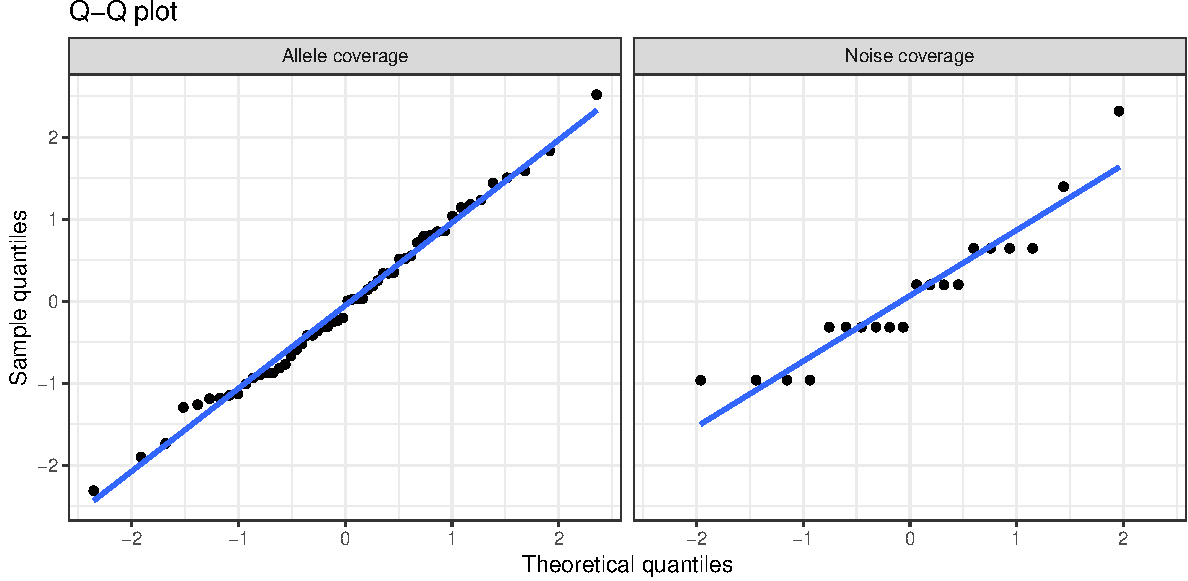
\includegraphics{MPSMixturesVignette_files/figure-latex/figQQ-1} 

}

\caption{\label{fig:qqtrue}Q-Q plot of the fitted model for both the allele and noise coverage models.}\label{fig:figQQ}
\end{figure}

\begin{figure}[ht!]

{\centering 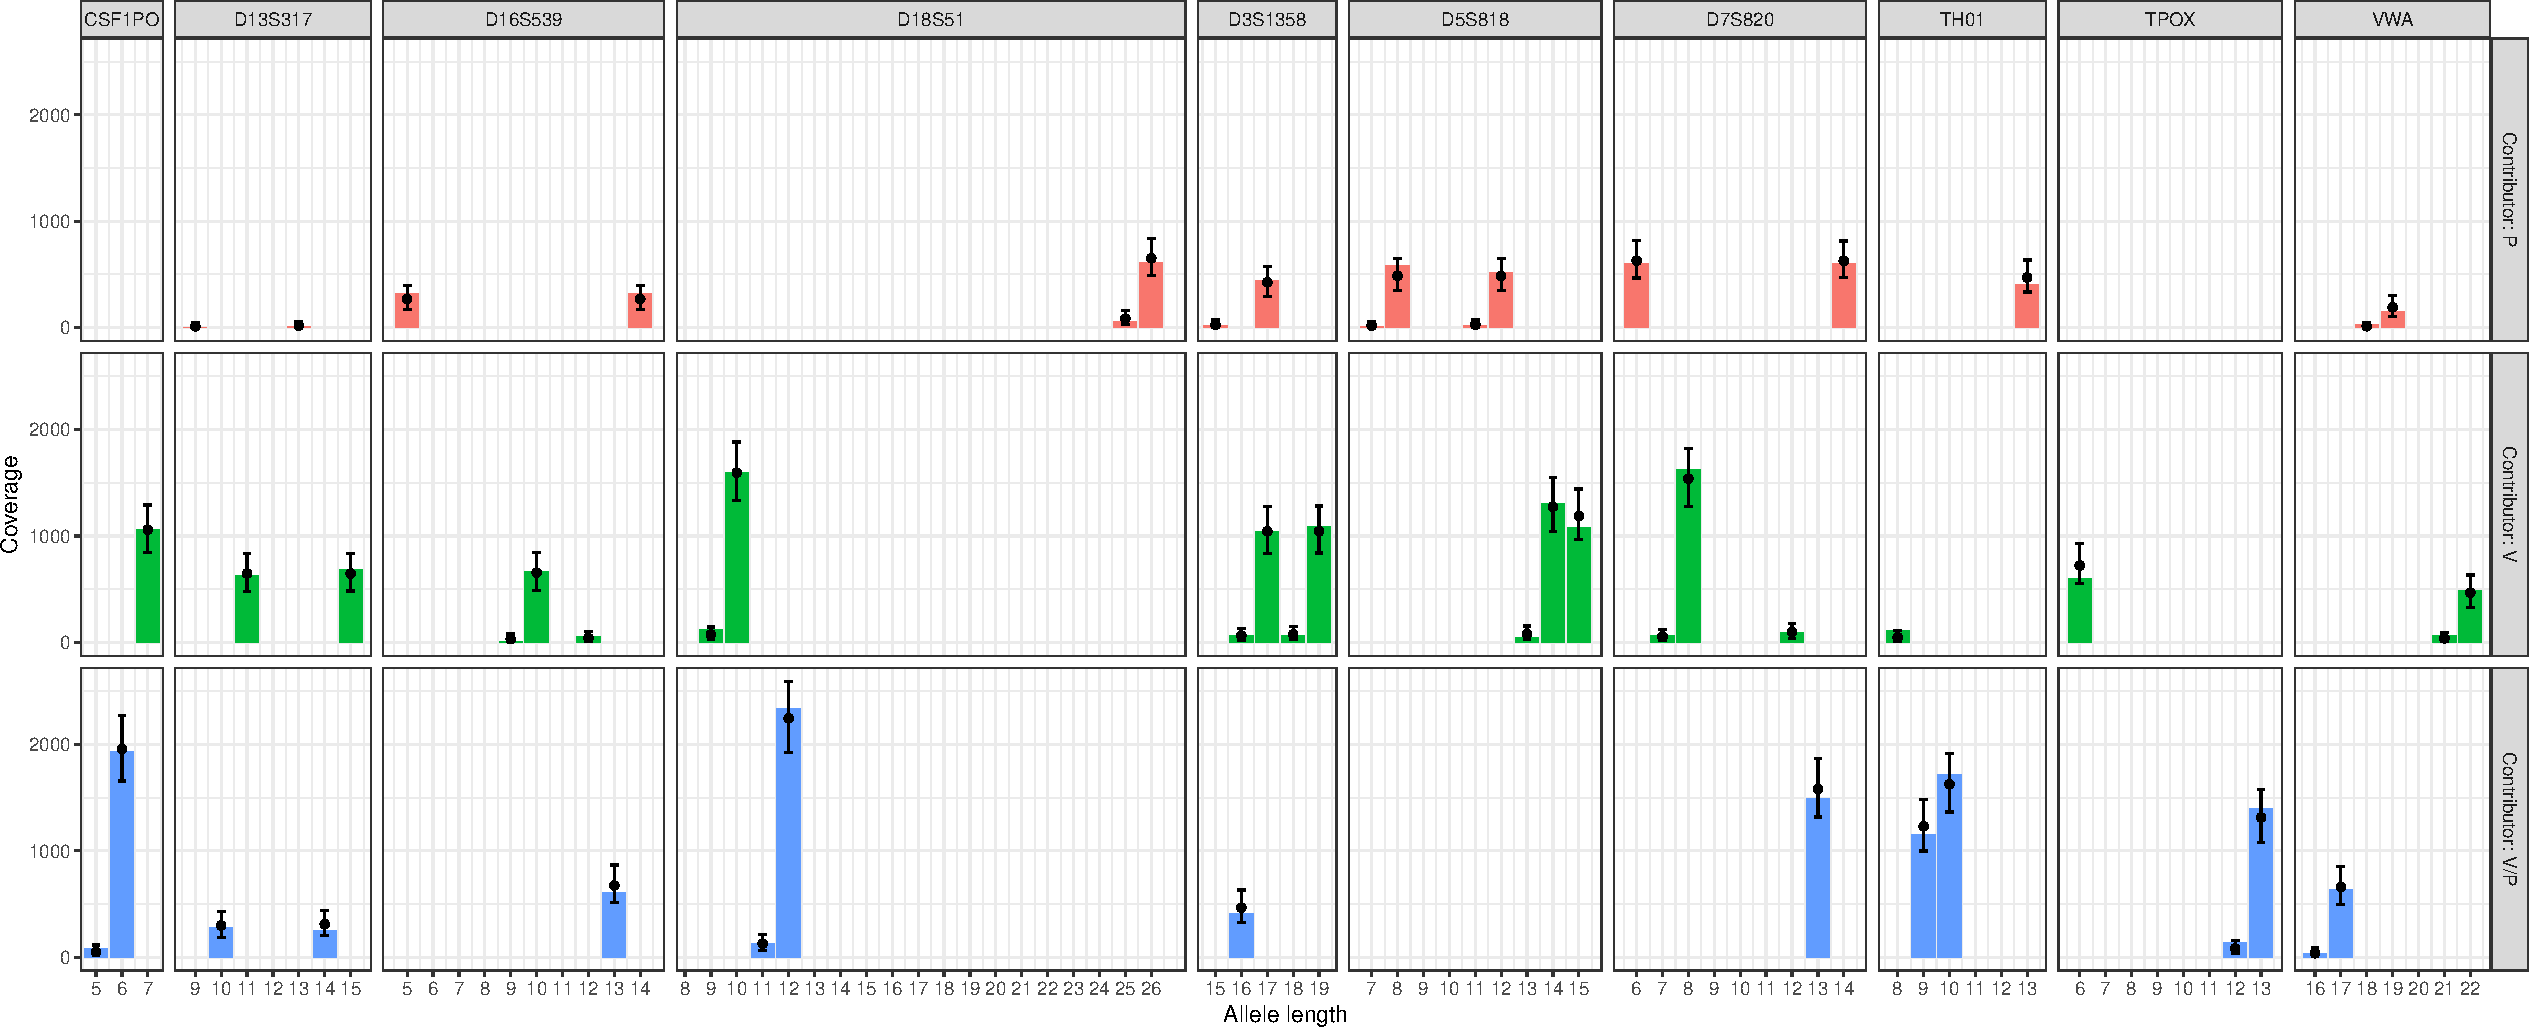
\includegraphics{MPSMixturesVignette_files/figure-latex/figEC-1} 

}

\caption{\label{fig:ectrue}Bar-plot of the coverage against the allele length for the each marker and profile, shown in coloumns and rows, respectively. Furthermore, the prediction interval for each observation is seen as the black bars, with the expected coverage at their center.}\label{fig:figEC}
\end{figure}

\subsection{Finding the best combination of unknown
genotypes}\label{sec:maximalUnknown}

As two is the total number of contributors, we have three possible
spaces of unknown genotypes. The spaces, when (1) the minor
(perpetrator) is known, (2) the major (victim) is known, and (3) both
contributors are unknown.

We will take each case in turn, trying to ascertain the optimal genotype
(or combination of genotypes), under the model. Furthermore, we will,
only in the first case, use both a single population and multiple
population model. In cases two and three, we will stick to the multiple
population approach, as it is more than ten times faster.

Note that if the genotypic information (allele frequencies) in the
population should be ignored, we can set \(\theta < 0\) or set all
allele frequencies to zero.

\subsubsection{Known minor}\label{known-minor}

We create an hypothesis using the \texttt{setHypothesis} function. The
known profiles should passed as a list containing an element for each of
the known profiles (in this case the perpetrator).

\begin{Shaded}
\begin{Highlighting}[]
\NormalTok{knownPerpetrator <-}\StringTok{ }\KeywordTok{setHypothesis}\NormalTok{(sampleTibble, numberOfContributors, trueProfiles[}\StringTok{"P"}\NormalTok{], theta)}
\end{Highlighting}
\end{Shaded}

We start with the single population algorithm:

\begin{Shaded}
\begin{Highlighting}[]
\NormalTok{controlSinglePopulation <-}\StringTok{  }
\StringTok{    }\KeywordTok{optimalUnknownProfileCombination.control}\NormalTok{(}
        \DataTypeTok{numberOfPopulations =} \DecValTok{1}\NormalTok{, }\DataTypeTok{numberOfIterations =} \DecValTok{350}\NormalTok{,}
        \DataTypeTok{populationSize =} \DecValTok{2000}\NormalTok{, }\DataTypeTok{numberOfFittestIndividuals =} \DecValTok{1}\NormalTok{,}
        \DataTypeTok{mutationDecayRate =} \DecValTok{1}\NormalTok{, }\DataTypeTok{hillClimbingIterations =} \DecValTok{0}\NormalTok{, }
        \DataTypeTok{parentSelectionWindowSize =} \DecValTok{15}\NormalTok{,}
        \DataTypeTok{allowParentSurvival =} \OtherTok{TRUE}\NormalTok{, }\DataTypeTok{trace =}\NormalTok{ F, }
        \DataTypeTok{levelsOfStutterRecursion =} \DecValTok{1}\NormalTok{, }
        \DataTypeTok{numberOfIterationsEqualMinMax =} \DecValTok{10}\NormalTok{, }
        \DataTypeTok{tolerance =} \KeywordTok{rep}\NormalTok{(}\FloatTok{1e-8}\NormalTok{, }\DecValTok{4}\NormalTok{)}
\NormalTok{    )}

\NormalTok{singlePopulationBenchmarkMajor <-}\StringTok{ }\KeywordTok{microbenchmark}\NormalTok{(}
\NormalTok{    optimalSingleMajor <-}\StringTok{ }
\StringTok{        }\KeywordTok{optimalUnknownProfileCombination}\NormalTok{(}\DataTypeTok{sampleTibble =}\NormalTok{ sampleTibble, }
                                         \DataTypeTok{markerImbalances =}\NormalTok{ markerImbalances, }
                                         \DataTypeTok{H =}\NormalTok{ knownPerpetrator[[}\DecValTok{1}\NormalTok{]], }
                                         \DataTypeTok{potentialParentsList =}\NormalTok{ potentialParentsList, }
                                         \DataTypeTok{control =}\NormalTok{ controlSinglePopulation),}
    \DataTypeTok{times =} \DecValTok{1}\NormalTok{)}
\end{Highlighting}
\end{Shaded}

The single population algorithm terminated in 3446.98 seconds.

The fittest found individual is always listed as the first entry in the
returned list. In this case, the log-likelihood in the fittest found
individual is -319.0504, with the log-likelihoods of the allele, noise,
and genotype probabilities at -279.2227, -39.8277, and 0. That is, the
found major contributor is the same as the true major contributor and
the increase in fitness is solely due to the added uncertainty
represented by the genotype probability. The corresponding estimated
parameters are (the same as seen above):

\begin{Shaded}
\begin{Highlighting}[]
\NormalTok{optimalSingleMajor}\OperatorTok{$}\NormalTok{U[[}\DecValTok{1}\NormalTok{]][[}\StringTok{"Parameters"}\NormalTok{]]}
\end{Highlighting}
\end{Shaded}

\begin{verbatim}
## $SampleParameters
## [1] 1379.690230    7.144928
## 
## $MixtureParameters
## [1] 0.294599 0.705401
## 
## $MarkerImbalanceParameters
##  [1] 0.9890816 0.6993384 0.6743920 1.4493215 1.0988994 1.2139757 1.5802224
##  [8] 1.1448998 0.6971334 0.4527359
## 
## $NoiseParameters
## [1] 3.698953e+00 9.078042e+01 2.000000e-16
\end{verbatim}

The relative difference for the parameters \(\nu\), \(\gamma\),
\(\psi\), \(\rho\), and \(\bs \varphi\) are given as: 0.01, 0.11, 0.23,
44.39, and 0.02, respectively. We see that the \(\hat \nu\),
\(\hat \gamma\), \(\hat \psi\), and \(\hat{\bs \varphi}\) are all within
10\% of the true values, only the overdispersion parameter of the noise
distribution, \(\hat \rho\), has proven difficult to estiamte.

We will use 32 sub-populations spread on four cores. Furthermore, we set
the size of each population to 75, i.e.~a total population size of
2,400.

\begin{Shaded}
\begin{Highlighting}[]
\NormalTok{controlMultiplePopulation <-}\StringTok{ }
\StringTok{    }\KeywordTok{optimalUnknownProfileCombination.control}\NormalTok{(}
        \DataTypeTok{numberOfPopulations =} \DecValTok{32}\NormalTok{, }\DataTypeTok{numberOfIterations =} \DecValTok{100}\NormalTok{,}
        \DataTypeTok{populationSize =} \DecValTok{75}\NormalTok{, }\DataTypeTok{numberOfFittestIndividuals =} \DecValTok{1}\NormalTok{,}
        \DataTypeTok{numberOfIterationsEqualMinMax =} \DecValTok{10}\NormalTok{,}
        \DataTypeTok{mutationDecayRate =} \DecValTok{1}\NormalTok{, }\DataTypeTok{hillClimbingIterations =} \DecValTok{0}\NormalTok{, }
        \DataTypeTok{parentSelectionWindowSize =} \DecValTok{6}\NormalTok{,}
        \DataTypeTok{allowParentSurvival =} \OtherTok{TRUE}\NormalTok{, }\DataTypeTok{trace =}\NormalTok{ F, }
        \DataTypeTok{levelsOfStutterRecursion =} \DecValTok{1}\NormalTok{, }
        \DataTypeTok{tolerance =} \KeywordTok{rep}\NormalTok{(}\FloatTok{1e-8}\NormalTok{, }\DecValTok{4}\NormalTok{)}
\NormalTok{    )}

\NormalTok{multiplePopulationBenchmarkMajor <-}\StringTok{ }\KeywordTok{microbenchmark}\NormalTok{(}
\NormalTok{    optimalMultipleMajor <-}\StringTok{ }
\StringTok{        }\KeywordTok{optimalUnknownProfileCombination}\NormalTok{(}\DataTypeTok{sampleTibble =}\NormalTok{ sampleTibble, }
                                         \DataTypeTok{markerImbalances =}\NormalTok{ markerImbalances, }
                                         \DataTypeTok{H =}\NormalTok{ knownPerpetrator[[}\DecValTok{1}\NormalTok{]], }
                                         \DataTypeTok{potentialParentsList =}\NormalTok{ potentialParentsList, }
                                         \DataTypeTok{control =}\NormalTok{ controlMultiplePopulation),}
    \DataTypeTok{times =} \DecValTok{1}\NormalTok{)}

\KeywordTok{save}\NormalTok{(optimalMultipleMajor, }\DataTypeTok{file =} \StringTok{"../inst/extdata/multipleMajor.RData"}\NormalTok{)}
\KeywordTok{save}\NormalTok{(multiplePopulationBenchmarkMajor, }\DataTypeTok{file =} \StringTok{"../inst/extdata/multipleMajorBench.RData"}\NormalTok{)}
\end{Highlighting}
\end{Shaded}

The parallel EA terminated in 2437.26 seconds, i.e.~close to ten times
faster than the single population algorithm. Thus, we see both an
increased performance from the parallelisation and the reduction in
population size. Furthermore, the fittest found individual had a fitness
of -319.0504. That is, the two approaches have terminated with the same
individual as the fittest individual.

In both cases the log-likehoods and fitness of the fittest individual
are given as:

\begin{Shaded}
\begin{Highlighting}[]
\NormalTok{optimalMultipleMajor}\OperatorTok{$}\NormalTok{U[[}\DecValTok{1}\NormalTok{]][}\KeywordTok{c}\NormalTok{(}\StringTok{"LogLikelihoods"}\NormalTok{, }\StringTok{"Fitness"}\NormalTok{, }\StringTok{"Parameters"}\NormalTok{)]}
\end{Highlighting}
\end{Shaded}

\begin{verbatim}
## $LogLikelihoods
## [1] -279.2227  -39.8277    0.0000
## 
## $Fitness
## [1] -319.0504
## 
## $Parameters
## $Parameters$SampleParameters
## [1] 1379.690230    7.144928
## 
## $Parameters$MixtureParameters
## [1] 0.294599 0.705401
## 
## $Parameters$MarkerImbalanceParameters
##  [1] 0.9890816 0.6993384 0.6743920 1.4493215 1.0988994 1.2139757 1.5802224
##  [8] 1.1448998 0.6971334 0.4527359
## 
## $Parameters$NoiseParameters
## [1] 3.698953e+00 9.078042e+01 2.000000e-16
\end{verbatim}

As the parallel EA was both faster and got the exact same result, we
will, in the remainder of this manuscript, only use the parallel EA.

\subsubsection{Known major}\label{known-major}

Now let us assume that the major is known (i.e.~the victim):

\begin{Shaded}
\begin{Highlighting}[]
\NormalTok{knownVictim <-}\StringTok{ }\KeywordTok{setHypothesis}\NormalTok{(sampleTibble, numberOfContributors, trueProfiles[}\StringTok{"V"}\NormalTok{], theta)}
\end{Highlighting}
\end{Shaded}

We will use the same control settings,
\texttt{controlMultiplePopulation}, as in the previous section.

\begin{Shaded}
\begin{Highlighting}[]
\NormalTok{optimalMultipleMinor <-}\StringTok{ }\KeywordTok{optimalUnknownProfileCombination}\NormalTok{(}\DataTypeTok{sampleTibble =}\NormalTok{ sampleTibble,}
                                                         \DataTypeTok{markerImbalances =}\NormalTok{ markerImbalances, }
                                                         \DataTypeTok{H =}\NormalTok{ knownVictim[[}\DecValTok{1}\NormalTok{]], }
                                                         \DataTypeTok{potentialParentsList =}\NormalTok{ potentialParentsList, }
                                                         \DataTypeTok{control =}\NormalTok{ controlMultiplePopulation)}
\end{Highlighting}
\end{Shaded}

The parameters, log-likelihoods, and fitness are:

\begin{Shaded}
\begin{Highlighting}[]
\NormalTok{optimalMultipleMinor}\OperatorTok{$}\NormalTok{U[[}\DecValTok{1}\NormalTok{]][}\KeywordTok{c}\NormalTok{(}\StringTok{"Parameters"}\NormalTok{, }\StringTok{"LogLikelihoods"}\NormalTok{, }\StringTok{"Fitness"}\NormalTok{)]}
\end{Highlighting}
\end{Shaded}

\begin{verbatim}
## $Parameters
## $Parameters$SampleParameters
## [1] 1379.757609    7.145342
## 
## $Parameters$MixtureParameters
## [1] 0.7054012 0.2945988
## 
## $Parameters$MarkerImbalanceParameters
##  [1] 0.9890816 0.6993384 0.6743920 1.4493215 1.0988994 1.2139757 1.5802224
##  [8] 1.1448998 0.6971334 0.4527359
## 
## $Parameters$NoiseParameters
## [1] 3.698953e+00 9.078042e+01 2.000000e-16
## 
## 
## $LogLikelihoods
## [1] -279.2226  -39.8277    0.0000
## 
## $Fitness
## [1] -319.0503
\end{verbatim}

Comparing the log-likelihoods of the optimal minor contributor to those
of the true profile, we see that the log-likelihood of the noise model
does not change, while the log-likelihood of the allele coverage is
smaller for the optimal minor than for the true minor. However, we see
that the decrease in the log-likehood allele coverage is outweighed by
an increase in the genotype probability.

\subsubsection{Both profiles unknown}\label{both-profiles-unknown}

Lastly, we assumed that both the profiles were unknown. This is
indicated by supplying an empty list (or just \texttt{NULL}) to the
knownProfiles argument. Furthermore, we have increased the number of
sub-populations, the population size, allowed for more outer
itertations, and increased the termination counter
\texttt{numberOfIterationsEqualMinMax}, giving the algorithm more times
to search the space.

\begin{Shaded}
\begin{Highlighting}[]
\NormalTok{bothUnknown <-}\StringTok{ }\KeywordTok{setHypothesis}\NormalTok{(sampleTibble, numberOfContributors, }\KeywordTok{list}\NormalTok{(), theta)}

\NormalTok{controlMultiplePopulation <-}\StringTok{ }
\StringTok{    }\KeywordTok{optimalUnknownProfileCombination.control}\NormalTok{(}
        \DataTypeTok{numberOfPopulations =} \DecValTok{64}\NormalTok{, }
        \DataTypeTok{numberOfIterations =} \DecValTok{100}\NormalTok{,}
        \DataTypeTok{populationSize =} \DecValTok{300}\NormalTok{,}
        \DataTypeTok{numberOfFittestIndividuals =} \DecValTok{1}\NormalTok{,}
        \DataTypeTok{numberOfIterationsEqualMinMax =} \DecValTok{50}\NormalTok{,}
        \DataTypeTok{hillClimbingIterations =} \DecValTok{0}\NormalTok{,}
        \DataTypeTok{mutationDecayRate =} \DecValTok{1}\NormalTok{,}
        \DataTypeTok{parentSelectionWindowSize =} \DecValTok{12}\NormalTok{,}
        \DataTypeTok{trace =} \OtherTok{FALSE}\NormalTok{, }
        \DataTypeTok{tolerance =} \KeywordTok{rep}\NormalTok{(}\FloatTok{1e-8}\NormalTok{, }\DecValTok{4}\NormalTok{)}
\NormalTok{    )}

\NormalTok{multiplePopulationBenchmarkUnknown <-}\StringTok{ }\KeywordTok{microbenchmark}\NormalTok{(}
\NormalTok{    optimalMultipleUnknown <-}\StringTok{ }
\StringTok{        }\KeywordTok{optimalUnknownProfileCombination}\NormalTok{(}\DataTypeTok{sampleTibble =}\NormalTok{ sampleTibble,}
                                         \DataTypeTok{markerImbalances =}\NormalTok{ markerImbalances,}
                                         \DataTypeTok{H =}\NormalTok{ bothUnknown[[}\DecValTok{1}\NormalTok{]],}
                                         \DataTypeTok{potentialParentsList =}\NormalTok{ potentialParentsList,}
                                         \DataTypeTok{control =}\NormalTok{ controlMultiplePopulation),}
    \DataTypeTok{times =} \DecValTok{1}\NormalTok{)}
\end{Highlighting}
\end{Shaded}

\begin{verbatim}
## Warning: Unknown or uninitialised column: 'Region'.
\end{verbatim}

The algorithm terminated in seconds. The parameters, log-likelihoods,
and fitness of the optimal unknown genotype combination is:

\begin{Shaded}
\begin{Highlighting}[]
\NormalTok{optimalMultipleUnknown}\OperatorTok{$}\NormalTok{U[[}\DecValTok{1}\NormalTok{]][}\KeywordTok{c}\NormalTok{(}\StringTok{"Parameters"}\NormalTok{, }\StringTok{"LogLikelihoods"}\NormalTok{, }\StringTok{"Fitness"}\NormalTok{)]}
\end{Highlighting}
\end{Shaded}

\begin{verbatim}
## $Parameters
## $Parameters$SampleParameters
## [1] 631.705707   6.775048
## 
## $Parameters$MixtureParameters
## [1] 0.98468955 0.01531045
## 
## $Parameters$MarkerImbalanceParameters
##  [1] 1.4517036 0.4775017 0.9264574 1.3345344 0.7299888 0.9403457 1.2593882
##  [8] 0.9973994 1.0588679 0.8238128
## 
## $Parameters$NoiseParameters
## [1] 552.2406806   1.0000000   0.1160502
## 
## 
## $LogLikelihoods
## [1] -177.4981 -231.7614    0.0000
## 
## $Fitness
## [1] -409.2595
\end{verbatim}

We see that the optimal combination of unknown genotypes is equal to the
true major and optimal minor, i.e.~the differences can be seen in Figure
\ref{fig:minor}. This, there was not a huge difference between the true
and the optimal genotype combinations, and as above the difference was
largely down to the allele frequencies of the population.

\subsection{Approximating the LR}\label{approximating-the-lr}

In our case of ficticious murder, we will assume that the victim is
known and its profile typed. We will define the following competing
hypotheses:

\begin{itemize}
\item The prosecution hypothesis, $\mc H_p$: The suspect, with genotype $\bs g_S$, is the perpetrator. 
\item The defence hypothesis, $\mc H_d$: Another random person from the population is the perpetrator.
\end{itemize}

In \texttt{R} we define a hypothesis by the \texttt{setHypothesis}
function. It takes the arguments: \texttt{sampleTibble}, the total
number of contributors to the mixture, \texttt{numberOfContributors}, a
list of the known profiles to the mixture, \texttt{knownProfilesList},
and the inbreeding coefficient, \texttt{theta}.

\begin{Shaded}
\begin{Highlighting}[]
\NormalTok{theta =}\StringTok{ }\DecValTok{0}
\NormalTok{knownProfilesHp <-}\StringTok{ }\NormalTok{trueProfiles}
\NormalTok{knownProfilesHd <-}\StringTok{ }\NormalTok{trueProfiles[}\StringTok{"V"}\NormalTok{]}

\NormalTok{Hp <-}\StringTok{ }\KeywordTok{setHypothesis}\NormalTok{(sampleTibble, numberOfContributors, knownProfilesHp, theta)}
\NormalTok{Hd <-}\StringTok{ }\KeywordTok{setHypothesis}\NormalTok{(sampleTibble, numberOfContributors, knownProfilesHd, theta)}
\end{Highlighting}
\end{Shaded}

An object of class \texttt{hypothesis} holds the total number of
contributors, the number of known contributors, the combined genotype
matrix of the known contributors, the inbreeding coefficient, and the
allele frequencies of the chosen population.

Given the \texttt{sampleTibble} and the two competing hypotheses, we can
initialise the EA for obtaining an approximate likelihood ratio by
calling the \texttt{LR} function. As before we run the parallel
algorithm with twelve sub-populations.

\begin{Shaded}
\begin{Highlighting}[]
\NormalTok{LRParallelPopulations <-}
\StringTok{    }\KeywordTok{LR}\NormalTok{(}\DataTypeTok{sampleTibble =}\NormalTok{ sampleTibble, }\DataTypeTok{Hp =}\NormalTok{ Hp, }\DataTypeTok{Hd =}\NormalTok{ Hd, }\DataTypeTok{markerImbalances =}\NormalTok{ markerImbalances,}
       \DataTypeTok{potentialParentsList =}\NormalTok{ potentialParentsList, }\DataTypeTok{stutterRatioModel =} \OtherTok{NULL}\NormalTok{,}
       \DataTypeTok{control =} \KeywordTok{optimalUnknownProfileCombination.control}\NormalTok{(}
           \DataTypeTok{numberOfPopulations =} \DecValTok{32}\NormalTok{, }\DataTypeTok{numberOfIterations =} \DecValTok{150}\NormalTok{,}
           \DataTypeTok{populationSize =} \DecValTok{75}\NormalTok{, }\DataTypeTok{numberOfFittestIndividuals =} \DecValTok{1000}\NormalTok{,}
           \DataTypeTok{hillClimbingIterations =} \DecValTok{0}\NormalTok{, }\DataTypeTok{mutationDecayRate =} \DecValTok{1}\NormalTok{,}
           \DataTypeTok{parentSelectionWindowSize =} \DecValTok{6}\NormalTok{, }\DataTypeTok{simplifiedReturn =} \OtherTok{FALSE}\NormalTok{,}
           \DataTypeTok{allowParentSurvival =} \OtherTok{TRUE}\NormalTok{, }\DataTypeTok{trace =} \OtherTok{FALSE}\NormalTok{, }
           \DataTypeTok{tolerance =} \KeywordTok{rep}\NormalTok{(}\FloatTok{1e-8}\NormalTok{, }\DecValTok{4}\NormalTok{)))}
\end{Highlighting}
\end{Shaded}

\begin{Shaded}
\begin{Highlighting}[]
\NormalTok{LRParallelPopulations <-}\StringTok{ }\KeywordTok{load_rdata}\NormalTok{(}\KeywordTok{system.file}\NormalTok{(}\StringTok{'extdata'}\NormalTok{, }\StringTok{"multipleLRMinor.RData"}\NormalTok{, }\DataTypeTok{package =} \StringTok{'MPSMixtures'}\NormalTok{))}
\end{Highlighting}
\end{Shaded}

The \texttt{hypothesis} class can take more than a single prosecutors or
defence hypothesis (and, therefore, so can the \texttt{LR} function),
and the \texttt{LR} function returns the likelihood ratios of every
pairwise comparison of these hypotheses. The comparison table is
accessed in the returned list as:

\begin{Shaded}
\begin{Highlighting}[]
\NormalTok{LRParallelPopulations}\OperatorTok{$}\NormalTok{ComparisonTable}
\end{Highlighting}
\end{Shaded}

\begin{verbatim}
##   Hp Hd  Log10LR
## 1  2  2 14.13637
\end{verbatim}

\section*{References}\label{references}
\addcontentsline{toc}{section}{References}

\hypertarget{refs}{}
\hypertarget{ref-Balding1994}{}
Balding, David J., and Richard, A. Nichols. 1994. ``DNA profile match
probability calculation: how to allow for population stratification,
relatedness, database selection and single bands.'' \emph{Forensic
Science International} 64: 125--40.

\hypertarget{ref-oyvind_bleka_2016}{}
Bleka, Øyvind., Geir Storvik, and Peter Gill. 2016. ``EuroForMix: An
open source software based on a continuous model to evaluate STR DNA
profiles from a mixture of contributors with artefacts.'' \emph{Forensic
Science International: Genetics} 21: 35--44.

\hypertarget{ref-cowell_etal_2015}{}
Cowell, Robert G., Therese Graversen, Steffen L. Lauritzen, and Julia
Mortera. 2015. ``Analysis of Forensic DNA Mixtures with Artefacts.''
\emph{Royal Statistical Society. Journal Series C: Applied Statistics}
64: 1--32.

\hypertarget{ref-steele_2016}{}
Steele, Christopher D., Matthew Greenhalgh, and David J. Balding. 2016.
``Evaluation of low-template DNA profiles using peak heights.''
\emph{Statistical Applications in Genetics and Molecular Biology} 15:
431--45.

\hypertarget{ref-taylor_etal_2013}{}
Taylor, Duncan, Jo-Anne Bright, and John S. Buckleton. 2013. ``The
interpretation of single source and mixed DNA profile.'' \emph{Forensic
Science International: Genetics} 7: 516--28.

\hypertarget{ref-tvedebrink_etal_2013}{}
Tvedebrink, Torben, Maria Asplund, Poul Svante Eriksen, Helle Smidt
Mogensen, and Niels Morling. 2013. ``Estimating drop-out probabilities
of STR alleles accounting for stutters, detection threshold truncation
and degradation.'' \emph{Forensic Science International: Genetics
Supplement Series} 4: e51--e52.

\hypertarget{ref-Vilsen2017b}{}
Vilsen, Søren B., Torben Tvedebrink, Poul Svante Eriksen, Helle Smidt
Mogensen, and Niels Morling. 2017. ``Analysing allelic drop-out in MPS
STR forensic genetics data.''


\end{document}
